

\chapter{Study of the PWD12 Sensor}
\label{chap:pwd12-study}

\section*{Introduction}

This chapter focuses on the Vaisala \gls{pwd12} visibility sensor, shown in figure~\ref{fig:pwd}, a key component to be integrated into the weather monitoring system. The study covers its functionality, measurement principles, supported features, and communication capabilities. Special attention is given to the configuration process, the command interface, and how the sensor behaves in standalone testing scenarios. Understanding the \gls{pwd12}’s capabilities and requirements is essential before proceeding with its integration into the broader system. This chapter establishes the technical basis for ensuring reliable operation and effective data acquisition. Unless otherwise specified, all technical details in this chapter are based on the Vaisala PWD22/52 User’s Guide \cite{vaisala2015pwd}.

\begin{figure}[H]
  \centering
  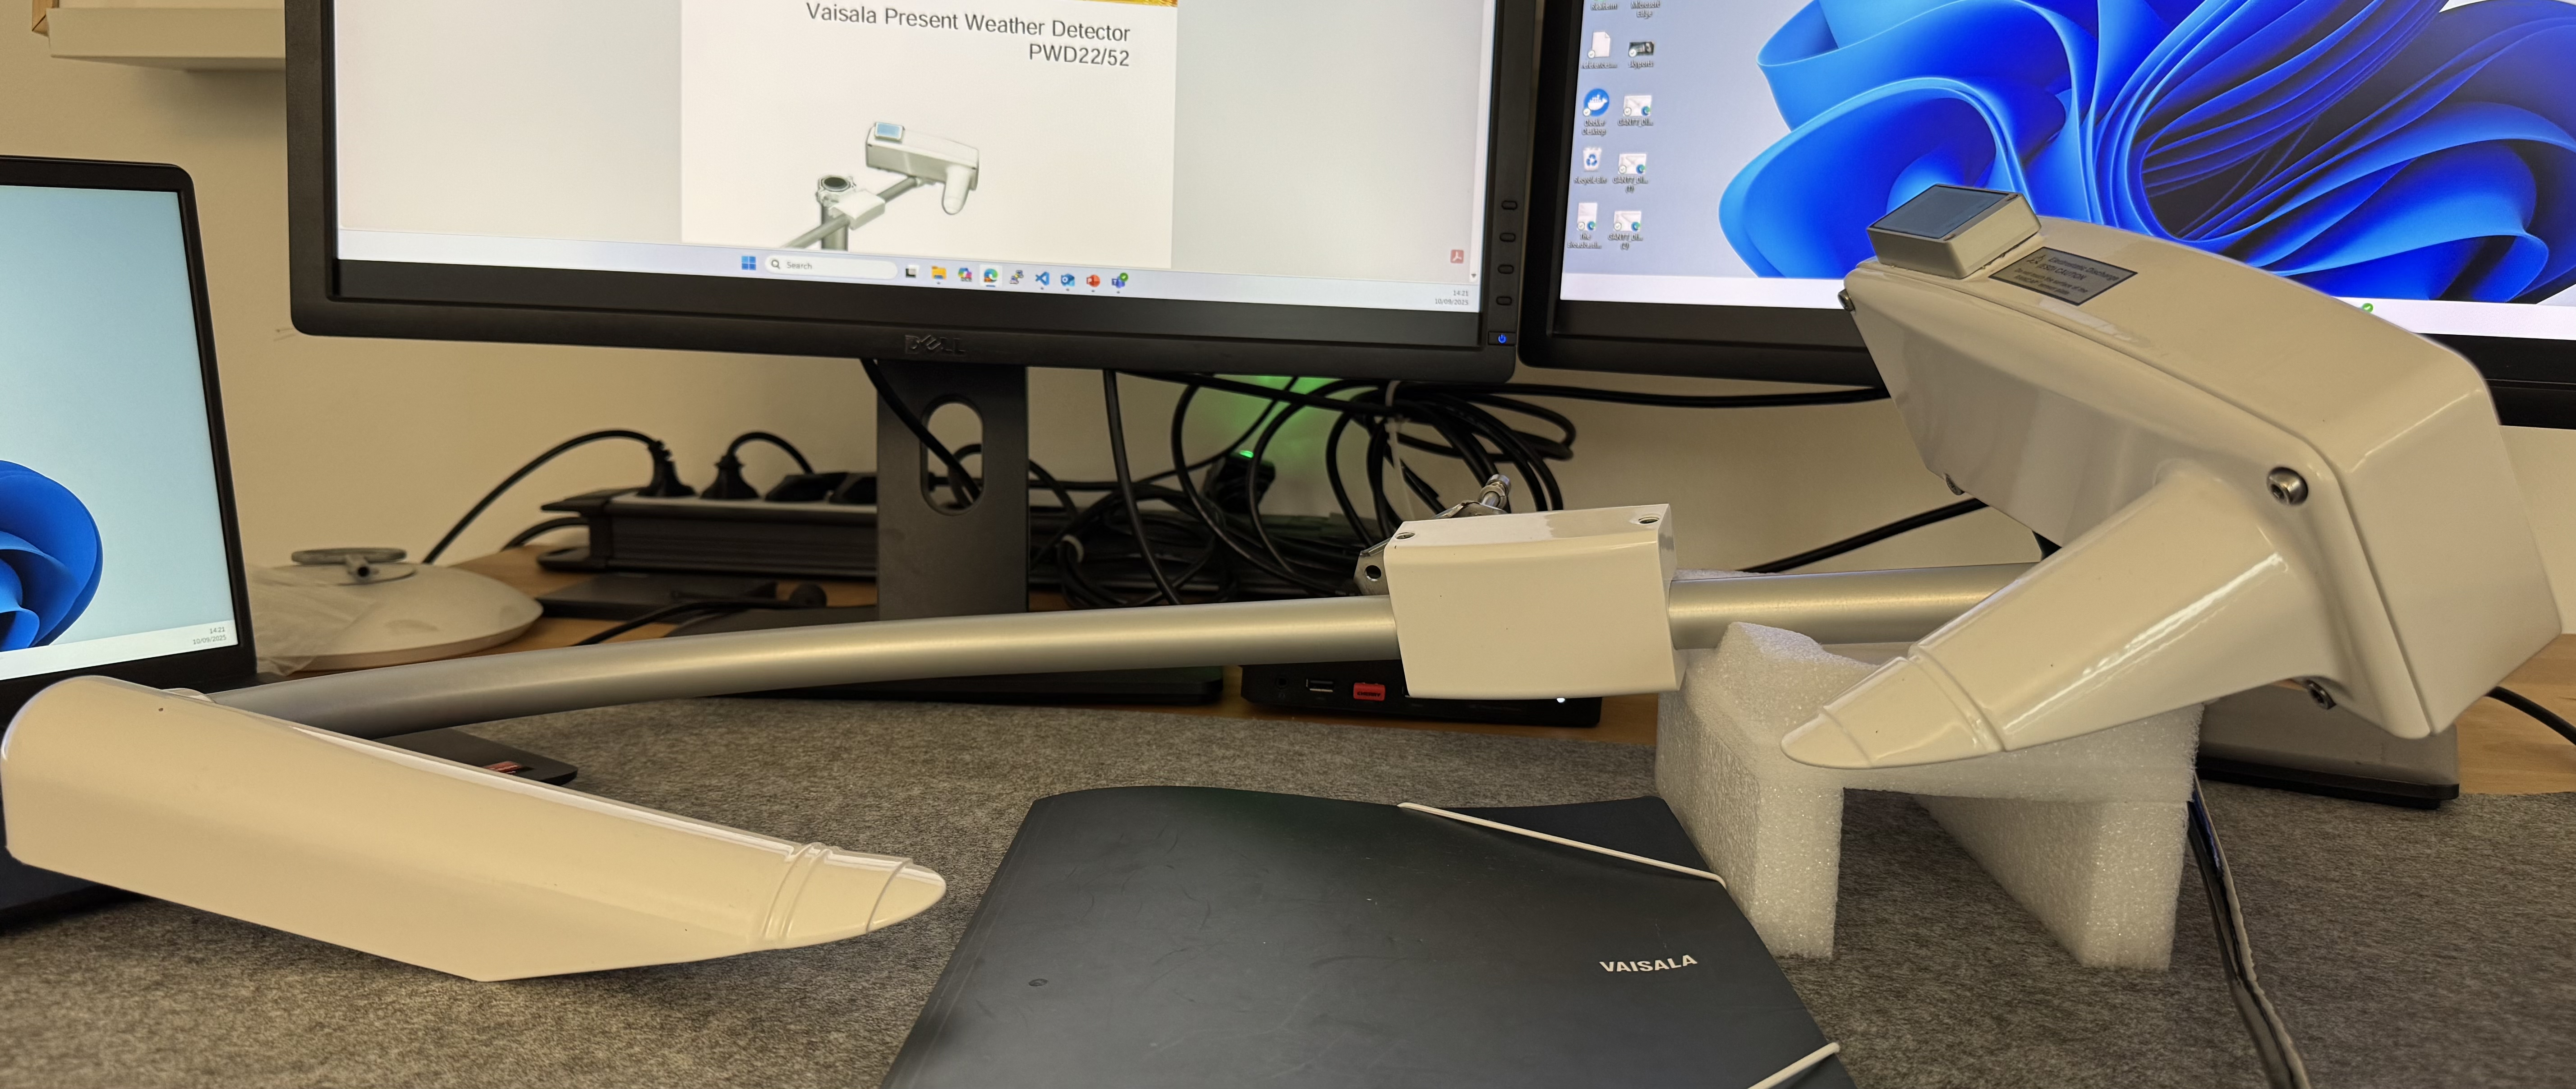
\includegraphics[width=1\textwidth]{images/Vaisala_PWD12.jpg}
  \caption{Vaisala Present Weather Detector PWD12}
  \label{fig:pwd}
\end{figure}

\section{Sensor Context and Operational Role}
\label{sec:pwd_context}

\subsection{Purpose of Integrating the PWD12}

The decision to integrate the \textbf{Vaisala \gls{pwd12}} visibility sensor into the weather station was largely influenced by Unisphere's prior experience with Vaisala hardware and the reliability of their certified instruments. Vaisala's long-standing reputation in meteorological sensing, combined with the sensor's compliance with aviation and meteorological standards, made it a trustworthy addition to the system. Although the decision was made before the start of the internship, the integration aligned well with the company's infrastructure and quality expectations.

\subsection{Role in the Weather Station}

The \gls{pwd12} extends the capabilities of the existing weather station by adding \textbf{visibility measurement}, a parameter that was not captured by the previously installed WXT536 sensor. This enhancement was essential for supporting operational environments such as vertiports, where visibility conditions directly impact the feasibility of air taxi operations.


\subsection{Relevance to UAS Operations and the NOVA Platform}

Visibility data plays a critical role in \textbf{\gls{uas}} operations, particularly under \textbf{\gls{vfr}} and for applications like \textbf{\gls{uam}}. In such contexts, poor visibility can ground flights or require re-routing, making accurate and localized measurement a key enabler for operational decision-making.

Within the NOVA platform, visibility readings contribute to weather-aware flight planning, real-time monitoring, and post-operation analysis. The integration of the \gls{pwd12} is especially relevant for advanced vertiport deployments, such as the one near \gls{dxb}, where air taxi services are planned. In these environments, visibility is not just a regulatory requirement but a critical factor in ensuring safety and operational continuity.



\section{Internal Architecture and Hardware Components}

The Vaisala \gls{pwd12} sensor is a sophisticated device designed to deliver precise visibility and present weather measurements in outdoor environments. This section explores its internal structure and the physical components that contribute to its functionality.

\subsection{Optical Measurement System}

At the core of the visibility measurement functionality is the \gls{pwd12}’s \textbf{forward-scatter optical system} \cite{vaisala2015pwd}. It consists of an infrared light source and a photodetector arranged at a 42° angle relative to each other. When light emitted by the source encounters airborne particles like fog or rain, some of the light is scattered and captured by the receiver. The intensity of this scattered light is used to calculate the \textbf{\gls{mor}}.

This arrangement allows for a compact design with minimal maintenance requirements, as it eliminates the need for moving parts. The measurement volume is carefully defined to avoid contamination from precipitation that may pass through but not reflect light effectively.

As shown in Figure \ref{fig:optic}, the layout of the optical components ensures that only forward-scattered light is measured, minimizing noise from ambient light and non-relevant angles.

\begin{figure}[H]
  \centering
  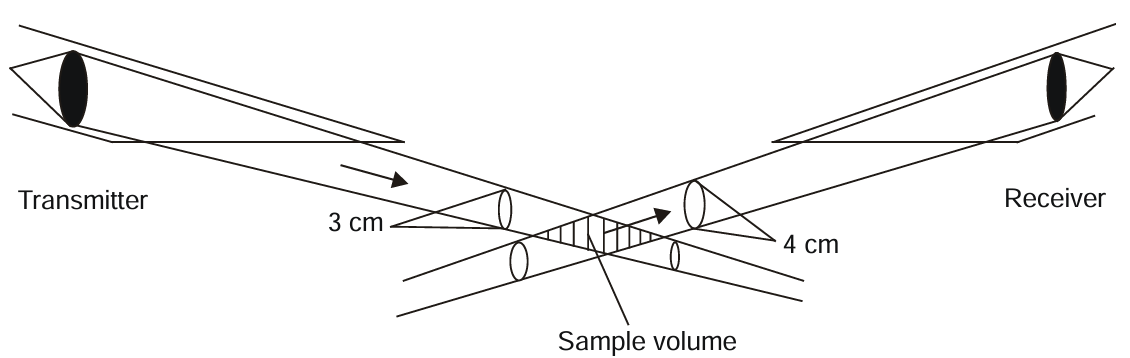
\includegraphics[width=0.9\textwidth]{images/optic.png}
  \caption{\gls{pwd12} Optical System Layout\cite{vaisala2015pwd}}
  \label{fig:optic}
\end{figure}

\subsection{RAINCAP Precipitation Sensor}

In parallel with visibility measurements, the \gls{pwd12} features a \textbf{RAINCAP} sensor\cite{vaisala2015pwd} mounted on the top of the enclosure. This is a solid-state capacitive sensor that detects precipitation through mechanical vibrations caused by raindrops or snowflakes hitting its surface. The internal signal processing algorithm analyzes the impact pattern and frequency to differentiate between precipitation types like drizzle, rain, snow, and sleet.

This mechanism allows for fast and reliable precipitation detection without requiring any moving parts, enhancing durability in the field. The design and principle of operation are illustrated in Figure \ref{fig:raincap}.

\begin{figure}[H]
  \centering
  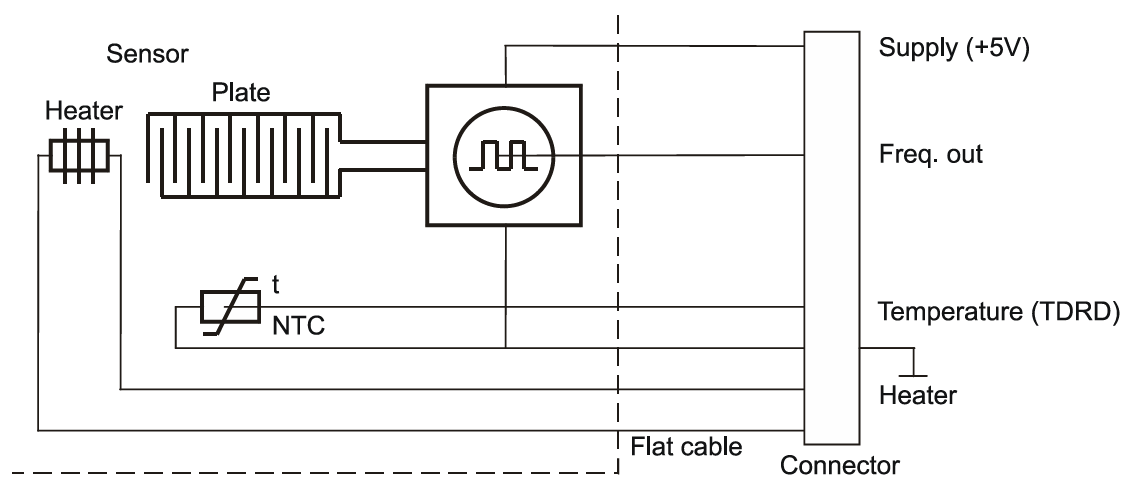
\includegraphics[width=0.9\textwidth]{images/raincap.png}
  \caption{RAINCAP Block Diagram\cite{vaisala2015pwd}}
  \label{fig:raincap}
\end{figure}

\subsection{Anti-Icing and Heating Mechanisms}

To ensure uninterrupted performance in cold and icy conditions, the \gls{pwd12} is equipped with \textbf{automatic heaters}\cite{vaisala2015pwd} located in three zones: the optical head, the RAINCAP sensor, and the main enclosure. These heaters are activated based on environmental conditions and internal temperature readings to prevent snow or ice buildup on sensitive areas.

The heater outputs can be controlled remotely via digital I/O lines or allowed to operate autonomously. The heater configuration helps maintain consistent measurement accuracy regardless of the surrounding weather.

\subsection{Signal Processing Unit and Embedded Controller}

All sensor outputs are processed by an embedded microcontroller inside the \gls{pwd12}. This unit is responsible for:
\begin{itemize}
    \item Converting raw analog signals into digital measurements,
    \item Filtering and applying classification algorithms,
    \item Generating weather codes and output strings,
    \item Managing communication and diagnostic reporting.
\end{itemize}

\subsubsection{Enclosure and Protection}

The Vaisala \gls{pwd12} is housed in a rugged, \textbf{\acrshort{ip66}-rated enclosure}\cite{vaisala2015pwd}, designed for long-term deployment in demanding outdoor environments. The enclosure combines \textbf{anodized aluminum} with \textbf{\acrshort{uv}-resistant polycarbonate} to ensure structural integrity, weather resistance, and longevity.

Key features of the protective design include:

\begin{itemize}
    \item \textbf{Ingress Protection:} The \gls{ip66} rating guarantees that the enclosure is dust-tight and protected against strong water jets from any direction, making it suitable for exposed locations.
    
    \item \textbf{\gls{emc} Shielding:} The internal electronics are shielded to comply with \textbf{\gls{en61326}}, reducing susceptibility to electrical interference from nearby equipment or power lines. This is essential when the sensor is installed near radar, communication antennas, or industrial machinery.
    
    \item \textbf{Grounding and Surge Protection:} A dedicated grounding terminal allows the sensor to be connected to the site’s earthing system. Additionally, the PWD12 includes internal protection components against electrostatic discharge and transient surges on communication and power lines. However, external surge arrestors are recommended for full compliance with installation best practices.
    
    \item \textbf{Environmental Robustness:} The physical form factor minimizes accumulation of snow, debris, or bird droppings on optical and sensing elements. The sloped housing design promotes self-cleaning, reducing maintenance needs.
    
    \item \textbf{Connector Interface:} The cable gland or M12 interface is sealed to prevent moisture ingress while providing mechanical strain relief for the cable.
\end{itemize}

These protection features make the \gls{pwd12} well-suited for aviation and meteorological applications where \textbf{continuous and interference-free operation} is essential.


\section{Technical Specifications}

The Vaisala \gls{pwd12} sensor is designed to provide high-accuracy visibility and present weather measurements. It outputs a variety of environmental parameters relevant for \gls{uas} operations, particularly under \gls{vfr} conditions.

\subsection{Measurable Parameters and Units}

The \gls{pwd12} outputs a rich set of weather data using periodic \gls{ascii} messages\cite{vaisala2015pwd}. The standard configuration includes the following measurements:
\begin{itemize}
    \item \textbf{Visibility}: 1-minute and 10-minute averaged visibility values (in meters).
    \item \textbf{Present Weather Codes}: Instantaneous, 15-minute, and 1-hour weather conditions using both \gls{nws} and \gls{wmo} code standards.
    \item \textbf{Precipitation}: Intensity (mm/h), cumulative precipitation (mm), and snow accumulation (mm).
    \item \textbf{Optional Parameters}: Air temperature (°C) and background luminance (cd/m²) can also be measured when Message 7 is enabled.
\end{itemize}


\subsection{Accuracy, Resolution, and Operating Ranges}

Table \ref{tab:pwd12specs} summarizes key performance parameters for the visibility and precipitation-related measurements\cite{vaisala2025pwd12}.
\begin{table}[H]
\small
\renewcommand{\arraystretch}{1.5}
\setlength{\tabcolsep}{8pt} % Adjust column padding

\centering
\caption{\gls{pwd12} Visibility Sensor Measurement Characteristics (See PWD Datasheet\cite{vaisala2025pwd12})}
\label{tab:pwd12specs}
\begin{tabular}{|p{3cm}|c|c|c|p{3.5cm}|}
    \hline
    \textbf{Parameter} & \textbf{Range} & \textbf{Interval} & \textbf{Uncertainty} & \textbf{Notes} \\
    \hline
    Visibility (1/10 min) & 1--2000 m & 15 s & ±10\% or ±2.5\% & Averaged over 1 and 10 minutes \\
    \hline
    Precipitation Intensity & 0--999.99 mm/h & 15 s & ±2.5\% & Resolution: 0.05 mm \\
    \hline
    Cumulative Precipitation & 0--99.99 mm & 15 s & ±2.5\% & Reset on restart or CLRS command \\
    \hline
    Snow Accumulation & 0--999 mm & 15 s & ±2.5\% & Reset on restart or CLRS command \\
    \hline
    Present Weather Code & 0--99 & 15 s & – & Based on optical and Doppler signals \\
    \hline
\end{tabular}
\end{table}

\subsection{Supported Message Types and Baud Rates}

The sensor is configured to emit \texttt{Message 2}, which contains the present weather status in standard format, and optionally \texttt{Message 7}\cite{vaisala2015pwd} for aviation-specific use. These messages are structured in the \gls{ascii} protocol and transmitted periodically over the \gls{rs485} interface.

Each message includes a \gls{crc} checksum for error detection, and consists of multiple comma-separated fields representing visibility, weather codes, precipitation levels, and optional extensions such as temperature and luminance.


\subsection{Power Requirements and Electrical Characteristics}

The \gls{pwd12} requires separate power inputs for its measurement electronics and its integrated heater system\cite{vaisala2015pwd}:

\begin{itemize}
    \item \textbf{Measurement Electronics:} 12–50\,V\,DC
    \item \textbf{Heaters:} 24\,V\,DC recommended
\end{itemize}

The sensor is designed for outdoor environments and includes built-in features for environmental resilience:
\begin{itemize}
    \item \textbf{Operating Temperature:} -40\textdegree{}C to +60\textdegree{}C
    \item \textbf{Ingress Protection:} \gls{ip66}-rated enclosure
    \item \textbf{\gls{emc} Protection:} The electronics comply with EN61326-1 and EN55011 Class B emission limits.
    \item \textbf{Mounting:} Vertical mounting with proper optical alignment (receiver facing north in the northern hemisphere).
\end{itemize}

\section{Installation and Environment Requirements}

Proper installation is crucial to ensure the long-term reliability, accuracy, and durability of the \gls{pwd12} sensor. Vaisala provides clear guidelines to mitigate environmental interference and support optimal sensor performance.

\subsection{Site Selection Guidelines}

The sensor must be installed in an open area with unobstructed airflow and visibility. According to Vaisala's recommendations\cite{vaisala2015pwd}:

\begin{itemize}
    \item A \textbf{minimum horizontal clearance of 100\,m} should be maintained from large objects such as buildings, trees, or towers.
    \item The sensor should not be mounted near heat sources (e.g., \gls{hvac} exhausts, rooftops) or highly reflective surfaces.
    \item The installation site must be accessible for maintenance and cleaning and support a vibration-free, rigid mounting base to minimize measurement artifacts.
\end{itemize}

Figure~\ref{fig:siteguidelines} from the official manual illustrates the optimal site selection constraints.

\begin{figure}[H]
    \centering
    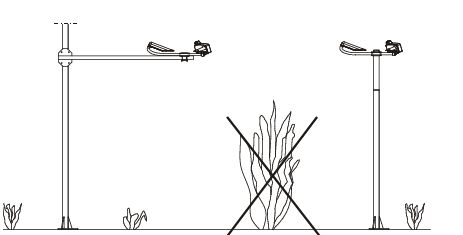
\includegraphics[width=0.75\textwidth]{images/loc.png}
    \caption{Recommended installation site criteria for PWD sensors (see PWD12 Manual\cite{vaisala2015pwd}, Chapter 4)}
    \label{fig:siteguidelines}
\end{figure}

\subsection{Mounting Orientation and Positioning}

The \gls{pwd12} is typically mounted on a vertical pole or mast using Vaisala's dedicated mounting kit\cite{vaisala2015pwd} or a compatible adapter. The optical head must remain perfectly horizontal during operation to avoid distortion in visibility measurement. The mounting setup should ensure:

\begin{itemize}
    \item A fixed, stable structure such as a mast or rail.
    \item Horizontal alignment of the sensor body and unobstructed view of the measurement volume.
    \item To avoid sunlight or artificial light interference, the optics should not face strong light sources.
    \item In the northern hemisphere, the \textbf{receiver should be oriented toward the north}, while in the southern hemisphere it should face south.
\end{itemize}

\subsection{Grounding and Surge Protection}

Electrical protection is essential, especially in outdoor installations exposed to lightning or power surges. Vaisala recommends the following protection measures\cite{vaisala2015pwd}:

\begin{itemize}
    \item The \gls{pwd12} sensor chassis must be \textbf{properly grounded} to earth using a dedicated grounding wire.
    \item A Vaisala \textbf{lightning protection device} should be installed in-line between the power source and the sensor, especially in high-risk areas.
    \item Shielded cables and grounded cable armor are recommended to further suppress electromagnetic interference.
\end{itemize}

Failing to implement grounding and surge protection can compromise both safety and long-term sensor performance.



\section{Electrical Wiring and Communication Interfaces}

The \gls{pwd12} sensor requires careful attention during electrical integration to ensure reliable communication and power delivery. This includes proper pin-out matching, interface selection, cable shielding, and adherence to electrical specifications. For complete wiring specifications, see the Vaisala PWD12 User Manual, Section 4.2\cite{vaisala2015pwd}.

\subsection{Pin-out and Wire Color Mapping}

The sensor is delivered with a fixed 16-wire cable, which provides lines for power, serial communication, relay outputs, and diagnostics. Table~\ref{tab:pwd12pins} shows the color mapping of the 16 wires in the \gls{pwd12} cable, the function of each wire, and the assigned pin:

\begin{table}[H]
\small
\renewcommand{\arraystretch}{1.5}
\centering
\caption{Recommended Pin-out Connections for Basic Operation}
\label{tab:pwd12pins}
\begin{tabular}{|c|l|l|}
\hline
\textbf{Wire Color} & \textbf{Function} & \textbf{Pin} \\
\hline
Red     & Power +24 VDC & 1 \\
\hline
Black   & Power GND     & 2 \\
\hline
White   & RS-485 B (-)     & 3 \\
\hline
Brown    & RS-485 A (+)     & 4 \\
\hline
Green    & RS-232 Tx      & 5 \\
\hline
Yellow  & RS-232 Rx  & 6 \\
\hline
Grey     & RS-232 GND & 7 \\
\hline
Blue   & Analog Output     & 8 \\
\hline
White/Green   & Heating Power +     & 9 \\
\hline
Brown/Green    & Heating Power +     & 10 \\
\hline
White/Yellow    & Heating Power -      & 11 \\
\hline
Brown/Yellow  & Heating Power -  & 12 \\
\hline
Grey/Pink   & Relay Control 1     & 13 \\
\hline
Red/Blue    & Relay Control 2     & 14 \\
\hline
Violet    & Relay Control 3 / Ext Vb      & 15 \\
\hline
Pink  & Ext Vb  & 16 \\
\hline
\end{tabular}
\end{table}

Figure~\ref{fig:pwd12pinouts} shows the full 16-pin connector layout that should be used in this installation.

\begin{figure}[H]
\centering
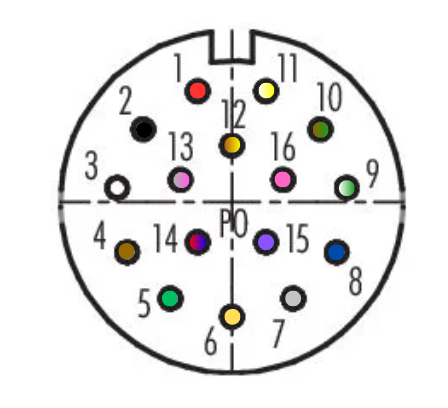
\includegraphics[width=0.4\textwidth]{images/16pins.png}
\caption{\gls{pwd12} cabling overview: 16-wire original mapping}
\label{fig:pwd12pinouts}
\end{figure}

\subsection{Supported Communication Interfaces}
\label{sec:pwd12wiring}

The \gls{pwd12} supports two digital communication interfaces:

\begin{itemize}
    \item \textbf{\gls{rs485} (default):} Full-duplex, differential communication. Recommended for long distances and electrically noisy environments. Baud rate: \textbf{9600}, \textbf{7 data bits}, \textbf{even parity}, \textbf{1 stop bit}.
    \item \textbf{\gls{rs232} (optional):} Used primarily for manual configuration and diagnostics. Requires a \gls{usb}–\gls{rs232} converter and a terminal emulator on the host device.
\end{itemize}

\textbf{RS-485 was selected for this integration} due to its superior resistance to electromagnetic interference, support for longer cable runs, and compatibility with existing RevPi serial interfaces. RS-232 was used only during initial bench testing and manual configuration.

\subsection{Cable Shielding and Length Constraints}

To ensure stable signal quality and \gls{emi} protection:

\begin{itemize}
    \item Use shielded twisted pair cables for \gls{rs485} signals.
    \item The cable shield (bare wire) should be grounded at the panel side only.
    \item Keep the communication cable length under \textbf{1,200 meters} for \gls{rs485}, as per standard limitations.
    \item Ensure separation between power lines and communication lines to reduce noise coupling.
\end{itemize}

These precautions improve data integrity and prevent \gls{crc} parsing errors in electrically noisy or outdoor environments\cite{vaisala2015pwd}.



\section{Sensor Configuration and Command Structure}

The Vaisala \gls{pwd12} sensor offers flexible configuration through a serial interface, primarily using \gls{rs232} for direct command access. Most configuration and diagnostic operations are executed in \textit{command mode}. The required serial parameters were outlined in Section~\ref{sec:pwd12wiring}, and this section focuses on the command protocol and available setup options.

During integration, the default settings were largely sufficient. Only minor adjustments were made to the output format (Message 2/7 selection), output interval, and filtering level using documented commands. All commands follow the syntax and descriptions provided in the Vaisala \gls{pwd12} User Manual (e.g., Section 7.3)\cite{vaisala2015pwd}.

\subsection{Command Mode and Access}

To access command mode via \gls{rs232}, the following command must be sent:

\begin{center}
    \texttt{OPEN *}
\end{center}

Once command mode is active, the sensor accepts \gls{ascii}-based instructions. All commands must be terminated with a carriage return (CR, \texttt{0x0D}). The sensor replies with either confirmation messages or returned data strings depending on the command type.

\subsection{Configuration and Setup Commands}

Table~\ref{tab:pwd12commands_config} summarizes common setup commands used to control sensor behavior and output characteristics.

\begin{table}[H]
\centering
\small
\renewcommand{\arraystretch}{1.4}
\caption{PWD12 Configuration Commands (see PWD12 Manual\cite{vaisala2015pwd}, Chap. 5)}
\label{tab:pwd12commands_config}
\begin{tabular}{|l|p{9cm}|}
\hline
\textbf{Command} & \textbf{Description} \\
\hline
\texttt{WSET} & View or modify weather message type and code format (NWS/WMO). \\
\hline
\texttt{SSET} & Configure output interval, filtering, and enabled parameters (e.g., temperature, luminance). \\
\hline
\texttt{CLRS} & Clear accumulated rain and snow measurements. Used at installation or reset. \\
\hline
\texttt{WPAR} & Display current weather-related parameters such as visibility, precipitation thresholds. \\
\hline
\texttt{MSG} & Select which output messages to emit (e.g., Message 2 or Message 7). \\
\hline
\end{tabular}
\end{table}

\subsection{Calibration and RAINCAP Adjustment}

The RAINCAP sensor can be recalibrated if necessary. Table~\ref{tab:pwd12commands_calibration} lists relevant commands.

\begin{table}[H]
\centering
\small
\renewcommand{\arraystretch}{1.4}
\caption{PWD12 RAINCAP Calibration Commands (see PWD12 Manual\cite{vaisala2015pwd}, Chap. 5)}
\label{tab:pwd12commands_calibration}
\begin{tabular}{|l|p{9cm}|}
\hline
\textbf{Command} & \textbf{Description} \\
\hline
\texttt{DRY ON} & Set reference level for no precipitation. Run when the sensor is dry. \\
\hline
\texttt{WET ON} & Set reference level for active precipitation. Run during rain. \\
\hline
\texttt{DRY} / \texttt{WET} & Read current dry/wet calibration status and thresholds. \\
\hline
\end{tabular}
\end{table}

\subsection{Diagnostic and Status Commands}

The sensor provides various commands to monitor internal status and ensure healthy operation:

\begin{table}[H]
\centering
\small
\renewcommand{\arraystretch}{1.4}
\caption{PWD12 Status and Diagnostic Commands (see PWD12 Manual\cite{vaisala2015pwd}, Chap. 5)}
\label{tab:pwd12commands_diag}
\begin{tabular}{|l|p{9cm}|}
\hline
\textbf{Command} & \textbf{Description} \\
\hline
\texttt{STAT} & Returns internal status and error flags. \\
\hline
\texttt{TEMP} & Displays current internal and ambient temperatures. \\
\hline
\texttt{IDN?} & Query the sensor’s model ID, firmware version, and serial number. \\
\hline
\end{tabular}
\end{table}

These diagnostic tools support field validation, health monitoring, and automated sensor management. Most of the commands listed above are covered in Section 7.3 and Appendix A of the PWD12 User Manual.

\paragraph{}%
Wherever possible, configuration changes were minimized to preserve factory-calibrated accuracy. The default Message 2 format and 15-second output interval proved sufficient for integration with the RevPi data pipeline and downstream GraphQL schema.


\section{Sensor Testing and Message Validation}

To ensure proper functionality and compatibility of the \gls{pwd12} sensor before integration into the operational weather station, it is essential to carry out standalone testing. This includes establishing a communication link, analyzing output message formats, and validating that all expected parameters are correctly reported and parsable.

\subsection{Bench Setup and Mock Communication}

For standalone testing outside of the field deployment, the \gls{pwd12} was connected to a controlled bench setup using a regulated laboratory power supply and a USB–RS485 converter attached to a development laptop. This allowed direct communication with the sensor before integrating it into the RevPi system.

The external power supply delivered 24\,V\,DC, sufficient to power the measurement electronics. Only the essential lines from the PWD12 16-wire cable were connected: power (red/black) and the differential pair for RS-485 communication (brown/white). The heaters and additional auxiliary lines were not used in this configuration.

Table~\ref{tab:pwd12benchpins} summarizes the connections made during the bench setup.

\begin{table}[H]
\renewcommand{\arraystretch}{1.6}
\centering
\small
\caption{Pin-out connections used for bench testing}
\label{tab:pwd12benchpins}
\begin{tabular}{|l|l|}
\hline
\textbf{PWD12 Wire Color} & \textbf{Function} \\
\hline
Red   & Power +24 VDC \\
\hline
Black & Power GND \\
\hline
Brown & RS-485 A (+) \\
\hline
White & RS-485 B (–) \\
\hline
\end{tabular}
\end{table}

Figure~\ref{fig:pwd12benchsetup} illustrates the simplified bench setup, showing the PWD12 sensor connected to the external power supply and to a laptop via USB–RS485 converter.

\begin{figure}[H]
  \centering
  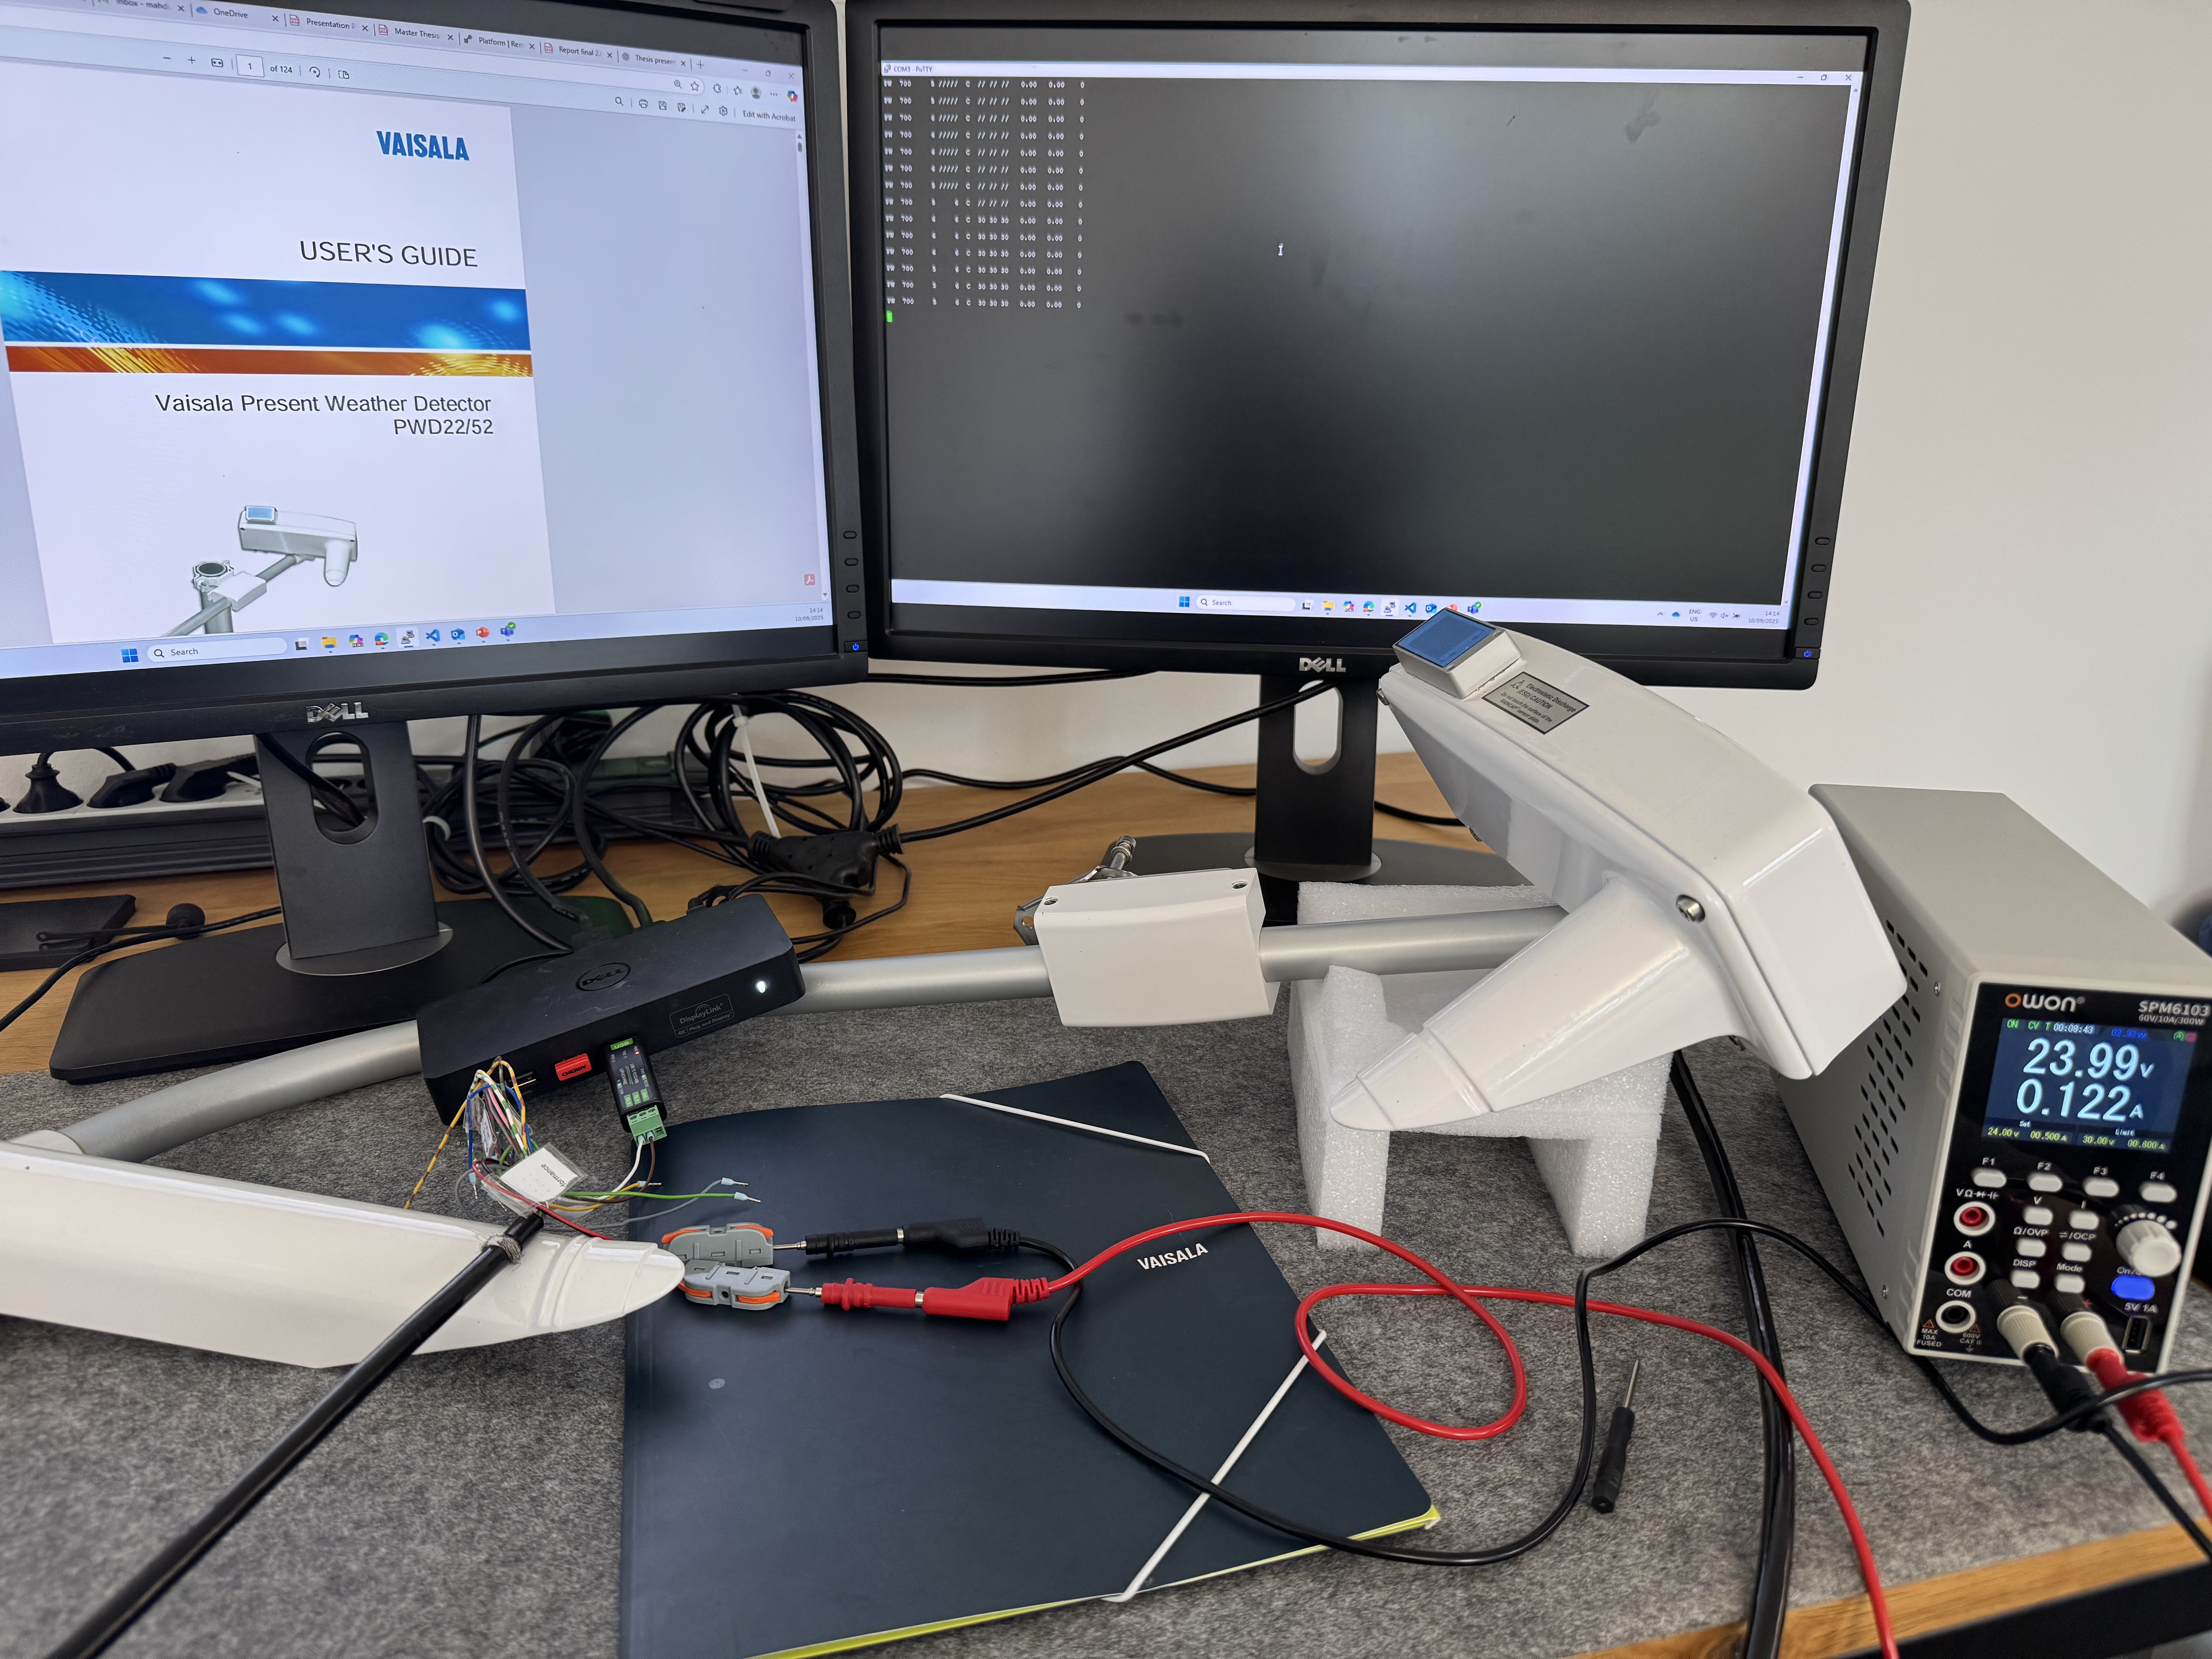
\includegraphics[width=0.7\textwidth]{images/pwd12_bench_setup.jpg} % <-- replace with your schematic
  \caption{Bench testing setup: PWD12 connected to external PSU and USB–RS485 converter}
  \label{fig:pwd12benchsetup}
\end{figure}

% \begin{table}[H]
% \renewcommand{\arraystretch}{1.8}
% \centering
% \caption{Pin-out Connections used for testing}
% \label{tab:pwd12testpins}
% \begin{tabular}{|c|l|l|l|}
% \hline
% \textbf{Wire Color} & \textbf{Function} & \textbf{M12 Pin} & \textbf{PWD12 Wire Color} \\
% \hline
% White     & ---                 & 1 & --- \\
% \hline
% Brown     & Power +24 VDC       & 2 & Red \\
% \hline
% Green     & ---                 & 3 & --- \\
% \hline
% Yellow    & ---                 & 4 & --- \\
% \hline
% Grey      & \gls{rs485} A (+)   & 5 & Brown \\
% \hline
% Pink      & ---                 & 6 & --- \\
% \hline
% Blue      & \gls{rs485} B (-)   & 7 & White \\
% \hline
% Red       & Power GND           & 8 & Black \\
% \hline
% \end{tabular}
% \end{table}

% Figure~\ref{fig:pwd12bench} shows the simplified 8-pin M12 connector layout used in the test bench.

% \begin{figure}[H]
%   \centering
%   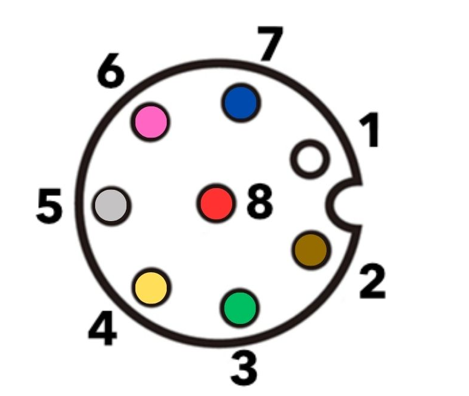
\includegraphics[width=0.5\textwidth]{images/8pins.png}
%   \caption{Simplified 8-pin wiring used for bench setup}
%   \label{fig:pwd12bench}
% \end{figure}

Before switching to VS Code, data was monitored using a terminal emulator (\texttt{Putty}), with serial settings matching the \gls{pwd12} specification: 9600 baud, 7 data bits, even parity, and 1 stop bit.

\subsection{Message Format Verification and Sensor Behavior}

Once powered and initialized, the \gls{pwd12} begins periodically transmitting data via the \gls{rs485} interface. By default, this output is in Message 2 format, which includes visibility readings, present weather codes, and precipitation data.

A representative message output is shown below:

\begin{verbatim}
PW 100 1839 1505 C 61 61 61 0.33 12.16 0
\end{verbatim}

Each field in the message corresponds to a specific parameter:

\begin{itemize}
  \item \texttt{PW} — Sensor prefix
  \item \texttt{1} — Sensor unit ID
  \item \texttt{00} — Status code
  \item \texttt{1839} — 1-minute average visibility (m)
  \item \texttt{1505} — 10-minute average visibility (m)
  \item \texttt{C} — Instant present weather (\gls{nws} code)
  \item \texttt{61, 61, 61} — Instant, 15-min, and 1-hour \gls{wmo} \gls{synop} weather codes
  \item \texttt{0.33} — Precipitation intensity (mm/h)
  \item \texttt{12.16} — Cumulative water sum (mm)
  \item \texttt{0} — Cumulative snow sum (mm)
\end{itemize}

During testing, this message was confirmed to:

\begin{itemize}
  \item Be emitted at the expected interval (typically every 15 seconds)
  \item Contain no malformed syntax or communication errors
  \item Include all expected measurement fields
\end{itemize}

\subsection{Raw Message Interpretation and Field Mapping}

To ensure compatibility with downstream processing and the cloud API, a dedicated Python parser was implemented to interpret raw messages. The parser handled:

\begin{itemize}
  \item Serial readout and newline stripping
  \item Splitting by whitespace
  \item Assigning each field to a semantically meaningful key
  \item Type validation (e.g., casting to float or integer)
\end{itemize}


\subsection{Final JSON Structure and Cloud Compatibility}

The parsed fields are serialized into a structured \gls{json} object as follows:

\begin{lstlisting}[language=json, caption={Parsed JSON structure from raw PWD12 message}, label={lst:parsedjson}]
{
  "sensor_id": "PW7",
  "visibility_alarm": "No Alarm",
  "status_code": "No hardware error",
  "visibility_1min": 1839,
  "visibility_10min": 1505,
  "present_weather_nws": "Light Rain",
  "present_weather_code_inst": "Rain",
  "present_weather_code_15min": "Rain",
  "present_weather_code_1h": "Rain",
  "precip_intensity": 0.33,
  "precip_cumulative": 12.16,
  "snow_sum": 0
}
\end{lstlisting}

This structure aligns with the expected GraphQL schema and supports direct ingestion by the cloud backend. The translation from \gls{wmo} and \gls{nws} codes to descriptive weather types is handled using predefined mapping tables.

Figure~\ref{fig:pwd12-raw-json} illustrates the transformation result: 
a raw ASCII message from the PWD12 sensor is parsed into a structured JSON object, 
aligning with the cloud schema for direct ingestion.

\begin{figure}[H]
  \centering
  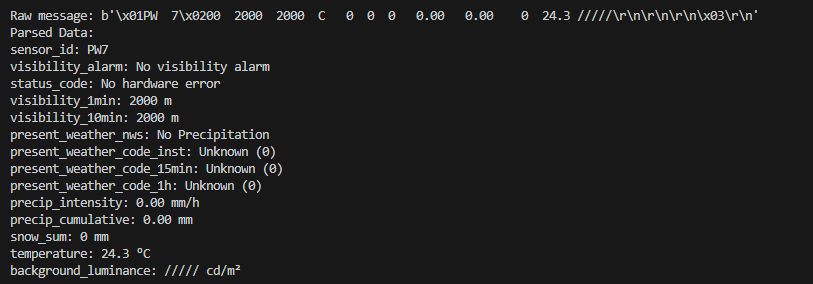
\includegraphics[width=\textwidth]{images/pwd12_raw_vs_json.png} % <-- your screenshot
  \caption{Example of a raw PWD12 message and the corresponding parsed JSON structure.}
  \label{fig:pwd12-raw-json}
\end{figure}


Additional parser logic ensures graceful failure handling for:

\begin{itemize}
  \item Incomplete messages or field truncation
  \item Unexpected data types
  \item Out-of-range values
\end{itemize}

This structured pipeline guarantees that data entering the cloud is both semantically valid and consistent across all weather stations.


\section*{Conclusion}

This chapter provided a comprehensive study of the Vaisala \gls{pwd12} sensor, outlining its measurement principles, internal components, technical specifications, and operational requirements. Particular emphasis was placed on understanding the optical forward-scatter method for visibility estimation, the RAINCAP precipitation detection system, and the role of integrated heating and protective mechanisms in ensuring continuous operation under harsh weather conditions.

Through standalone bench testing, the sensor’s communication interface and output format were successfully verified. Raw ASCII messages were captured, parsed, and transformed into structured JSON objects, demonstrating compatibility with downstream data handling pipelines. The tests confirmed that the sensor reliably outputs visibility, precipitation, and present weather codes at the expected intervals, with no communication errors or malformed data.

By establishing both the theoretical background and practical validation of the sensor’s output, this study laid the groundwork for its integration into the operational weather station. The findings ensure confidence that the \gls{pwd12} can extend the system’s capabilities with accurate visibility data, thereby supporting weather-aware flight monitoring and vertiport operations. The next chapter builds on these results by addressing the integration process, covering the hardware wiring, software architecture, and cloud connectivity required to deploy the sensor in the field.